% !TEX TS-program = pdflatex
% !TEX encoding = UTF-8 Unicode

% This is a simple template for a LaTeX document using the "article" class.
% See "book", "report", "letter" for other types of document.

\documentclass[11pt]{article} % use larger type; default would be 10pt


%%% PAGE DIMENSIONS
%\usepackage{geometry} % to change the page dimensions
%\geometry{a4paper} % or letterpaper (US) or a5paper or....
% \geometry{margin=2in} % for example, change the margins to 2 inches all round
% \geometry{landscape} % set up the page for landscape
%   read geometry.pdf for detailed page layout information
%\usepackage[textwidth=14cm,textheight=20cm]{geometry}
\usepackage[a4paper,%
            left=2.5cm,right=2.5cm,top=2.5cm,bottom=2.5cm,%
            footskip=.6cm]{geometry}

\def\changemargin#1#2{\list{}{\rightmargin#2\leftmargin#1}\item[]}
\let\endchangemargin=\endlist


\usepackage{graphicx} % support the \includegraphics command and options
\usepackage[parfill]{parskip} % Activate to begin paragraphs with an empty line rather than an indent


%%% PACKAGES
\usepackage{booktabs} % for much better looking tables
\usepackage{array} % for better arrays (eg matrices) in maths
\usepackage{paralist} % very flexible & customisable lists (eg. enumerate/itemize, etc.)
\usepackage{verbatim} % adds environment for commenting out blocks of text & for better verbatim
\usepackage{subfig} % make it possible to include more than one captioned figure/table in a single float
% These packages are all incorporated in the memoir class to one degree or another...


\usepackage{float}
\usepackage[all]{xy}
\usepackage{booktabs}
\usepackage{makecell}
\usepackage{enumerate}
\usepackage{scrextend}
\usepackage{mathtools}
\usepackage{yfonts}
\usepackage{setspace} 

\title{\LARGE Seminar zum Thema Numerische multilineare Algebra:\\
\LARGE Tensor Spaces and Numerical Tensor Calculus\\
\vspace{5mm} %5mm vertical space
\large Vortrag: Numerische Verfahren zur Bestimmung des Rangs eines Tensors}

\date{Vortrag vom 13.01.2020}

\author{Tibor Gr{\"u}n}


\makeatletter
% we use \prefix@<level> only if it is defined
\renewcommand{\@seccntformat}[1]{%
  \ifcsname prefix@#1\endcsname
    \csname prefix@#1\endcsname
  \else
    \csname the#1\endcsname\quad
  \fi}
% define \prefix@section
\newcommand\prefix@section{Kapitel \thesection: }
\makeatother


%%% For Math
\usepackage{amsmath}
\usepackage{amsfonts}
\usepackage{amsbsy}
\usepackage{amsthm}
\usepackage{amssymb}

\usepackage{mathtools}
\usepackage{commath}
\usepackage[sc,osf]{mathpazo}

\makeatletter
\renewcommand*\env@matrix[1][*\c@MaxMatrixCols c]{%
  \hskip -\arraycolsep
  \let\@ifnextchar\new@ifnextchar
  \array{#1}}
\makeatother

%%% Math theorem styles
\theoremstyle{definition}
\newtheorem{thm}{Satz}[section]
\newtheorem{lemma}[thm]{Lemma}
\newtheorem{definition}[thm]{Definition}
\newtheorem{rmk}[thm]{Bemerkung}
\newtheorem{alg}[thm]{Algorithmus}


%%% Math equation numbering
\numberwithin{equation}{section}

%%% For graphics
\usepackage{tikz}
\usepackage{pgfbaselayers}

\pgfdeclarelayer{background}
\pgfdeclarelayer{foreground}
\pgfsetlayers{background,main,foreground}


%%% For bibliography
\usepackage[utf8]{inputenc}
\usepackage[nottoc]{tocbibind}


%\DeclareMathOperator{\Hom}{Hom}
%\DeclareMathOperator{\dom}{dom}
%\DeclareMathOperator{\codom}{codom}

\begin{document}
	\pagenumbering{gobble}

	\maketitle

	\newpage

	\tableofcontents

	\newpage

	\pagenumbering{arabic}

\section{Tensoren}

%1.1
\subsection{Was ist ein Tensor?}

Im Folgenden sei $d \in \mathbb{Z}_{\geq 0}$ eine ganze Zahl, für $j \in \{1,\dots , d \}$, $n_{j} \in \mathbb{N}_{0}$
 natürliche Zahlen
und die Indexmengen $I_{j}$ endlich, also $I_{j} = \{1,\dots , n_{j} \}$. Alle Vektorräume $V_{j}$ seien über dem Körper $\mathbb{R}$,
also $V_{j} = \mathbb{R}^{I_{j}} =: \mathbb{R}^{n_{j}}$.

Für \textit{Tensoren} verwenden wir fettgedruckte Buchstaben $\mathbf{T}, \mathbf{S}, \mathbf{v}$; für Vektoren, aus
 denen sich die
Tensoren ergeben, kursive Buchstaben $v, T$. Die \textit{j}-te Dimension wird als Exponent hochgestellt, die Auswertung der
Einträge über die Indizes $i_{j}$ unten angestellt $v^{(j)}_{i_{j}}, T_{121}$ oder in eckigen Klammern angefügt $\mathbf{v}[i_{1},\dots,i_{d}]$.

%
% grafische Darstellung
\subsubsection{Vektoren, Matrizen, Tensoren: Grafische Darstellung \cite{tensor_networs_simons}}
\begin{changemargin}{0pt}{0pt}

Einen Tensor kann man folgendermaßen beschreiben: Es ist eine Box mit $d$ Antennen, die aus der Box herausragen.
Für jede Antenne $j$ ist eine Menge $I_{j}$ an Labels $i_{j} \in I_{j}$ möglich.
Wenn man an alle $d$ Antennen jeweils ein Label $i_{j}$ angebracht hat, kommt eine Zahl heraus.
\end{changemargin}

\begin{itemize}
\item
\begin{changemargin}{0pt}{0pt}
Zum Beispiel für $d=1, I_{1} = I = \{1,2,3\}$ und den Vektor $v = (7,5,3) \in \mathbb{R}^{3}$
können wir labeln mit $i = 1$, $i = 2$ oder $i = 3$:
\end{changemargin}

\begin{changemargin}{20pt}{20pt}
\begin{center}
\begin{minipage}{.2\textwidth}
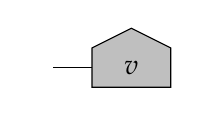
\begin{tikzpicture}
\begin{pgfonlayer}{foreground}
\draw[fill=lightgray] (0-0.5cm,0-0.25cm) -- (0+0.5cm,0-0.25cm) -- (0+0.5cm,0+0.25cm) -- (0,0+0.5cm) -- (0-0.5cm,0+0.25cm) -- cycle;
\node at (0,0) {$v$};
\end{pgfonlayer}
\begin{pgfonlayer}{background}
\draw[-] (0,0) -- (180:1cm);
\node at (180:1.2cm) { };
\end{pgfonlayer}
\end{tikzpicture}

\end{minipage}
%
\begin{minipage}{.2\textwidth}

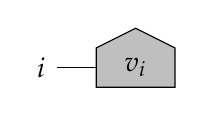
\begin{tikzpicture}
\begin{pgfonlayer}{foreground}
\draw[fill=lightgray] (0-0.5cm,0-0.25cm) -- (0+0.5cm,0-0.25cm) -- (0+0.5cm,0+0.25cm) -- (0,0+0.5cm) -- (0-0.5cm,0+0.25cm) -- cycle;
\node at (0,0) {$v_{i}$};
\end{pgfonlayer}
\begin{pgfonlayer}{background}
\draw[-] (0,0) -- (180:1cm);
\node at (180:1.2cm) {$i$};
\end{pgfonlayer}
\end{tikzpicture}

\end{minipage}
%
\begin{minipage}{.2\textwidth}
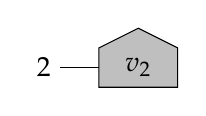
\begin{tikzpicture}
\begin{pgfonlayer}{foreground}
\draw[fill=lightgray] (0-0.5cm,0-0.25cm) -- (0+0.5cm,0-0.25cm) -- (0+0.5cm,0+0.25cm) -- (0,0+0.5cm) -- (0-0.5cm,0+0.25cm) -- cycle;
\node at (0,0) {$v_{2}$};
\end{pgfonlayer}
\begin{pgfonlayer}{background}
\draw[-] (0,0) -- (180:1cm);
\node at (180:1.2cm) {$2$};
\end{pgfonlayer}
\end{tikzpicture}

\end{minipage}
%
\begin{minipage}{.2\textwidth}
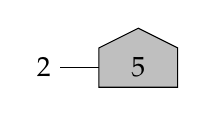
\begin{tikzpicture}
\begin{pgfonlayer}{foreground}
\draw[fill=lightgray] (0-0.5cm,0-0.25cm) -- (0+0.5cm,0-0.25cm) -- (0+0.5cm,0+0.25cm) -- (0,0+0.5cm) -- (0-0.5cm,0+0.25cm) -- cycle;
\node at (0,0) {$5$};
\end{pgfonlayer}
\begin{pgfonlayer}{background}
\draw[-] (0,0) -- (180:1cm);
\node at (180:1.2cm) {$2$};
\end{pgfonlayer}
\end{tikzpicture}
\end{minipage}
\end{center}
\end{changemargin}

\begin{changemargin}{0pt}{0pt}
Wir können also entweder kein Label anbringen, dann bleibt es ein Vektor, oder ein Label, dann kommt eine Zahl heraus.
\end{changemargin}

\item
\begin{changemargin}{0pt}{0pt}
Bei $d=2$ haben wir schon mehr Möglichkeiten. Entweder bei $j=1$ ein Label anbringen, oder bei $j=2$ oder bei beiden:
\end{changemargin}

\begin{changemargin}{20pt}{20pt}
\begin{center}
\begin{minipage}{.2\textwidth}
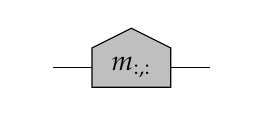
\begin{tikzpicture}
\begin{pgfonlayer}{foreground}
\draw[fill=lightgray] (0-0.5cm,0-0.25cm) -- (0+0.5cm,0-0.25cm) -- (0+0.5cm,0+0.25cm) -- (0,0+0.5cm) -- (0-0.5cm,0+0.25cm) -- cycle;
\node at (0,0) {$m_{:,:}$};
\end{pgfonlayer}
\begin{pgfonlayer}{background}
\draw[-] (0,0) -- (180:1cm);
\node at (180:1.2cm) { };
\draw[-] (0,0) -- (0:1cm);
\node at (0:1.2cm) { };
\end{pgfonlayer}
\end{tikzpicture}

\end{minipage}
%
\begin{minipage}{.2\textwidth}

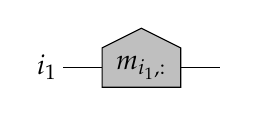
\begin{tikzpicture}
\begin{pgfonlayer}{foreground}
\draw[fill=lightgray] (0-0.5cm,0-0.25cm) -- (0+0.5cm,0-0.25cm) -- (0+0.5cm,0+0.25cm) -- (0,0+0.5cm) -- (0-0.5cm,0+0.25cm) -- cycle;
\node at (0,0) {$m_{i_{1},:}$};
\end{pgfonlayer}
\begin{pgfonlayer}{background}
\draw[-] (0,0) -- (180:1cm);
\node at (180:1.2cm) {$i_{1}$};
\draw[-] (0,0) -- (0:1cm);
\node at (0:1.2cm) { };
\end{pgfonlayer}
\end{tikzpicture}

\end{minipage}
%
\begin{minipage}{.2\textwidth}
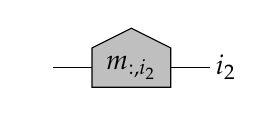
\begin{tikzpicture}
\begin{pgfonlayer}{foreground}
\draw[fill=lightgray] (0-0.5cm,0-0.25cm) -- (0+0.5cm,0-0.25cm) -- (0+0.5cm,0+0.25cm) -- (0,0+0.5cm) -- (0-0.5cm,0+0.25cm) -- cycle;
\node at (0,0) {$m_{:,i_{2}}$};
\end{pgfonlayer}
\begin{pgfonlayer}{background}
\draw[-] (0,0) -- (180:1cm);
\node at (180:1.2cm) { };
\draw[-] (0,0) -- (0:1cm);
\node at (0:1.2cm) {$i_{2}$};
\end{pgfonlayer}
\end{tikzpicture}

\end{minipage}
%
\begin{minipage}{.2\textwidth}
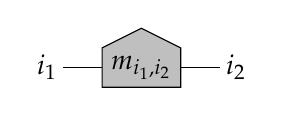
\begin{tikzpicture}
\begin{pgfonlayer}{foreground}
\draw[fill=lightgray] (0-0.5cm,0-0.25cm) -- (0+0.5cm,0-0.25cm) -- (0+0.5cm,0+0.25cm) -- (0,0+0.5cm) -- (0-0.5cm,0+0.25cm) -- cycle;
\node at (0,0) {$m_{i_{1},i_{2}}$};
\end{pgfonlayer}
\begin{pgfonlayer}{background}
\draw[-] (0,0) -- (180:1cm);
\node at (180:1.2cm) {$i_{1}$};
\draw[-] (0,0) -- (0:1cm);
\node at (0:1.2cm) {$i_{2}$};
\end{pgfonlayer}
\end{tikzpicture}
\end{minipage}
\end{center}
\end{changemargin}

\begin{changemargin}{0pt}{0pt}
Heraus kommt dann jeweils eine Matrix, ein Zeilenvektor, ein Spaltenvektor oder eine Zahl.
\end{changemargin}

\item

\begin{changemargin}{0pt}{0pt}
Dies lässt sich bei $d\geq3$ weiter verallgemeinern. Lässt man z.B. bei einem $4$-stufigen Tensor zwei Antennen frei,
und besetzt die anderen zwei mit Labeln, dann kommt wieder eine Matrix heraus.\\
Aus einem $3$-stufigen Tensor $\mathbf{T} \in \mathbb{R}^{I_{1}\times I_{2} \times I_{3}}$ kann man auf drei verschiedene Arten eine Matrix machen:
\end{changemargin}
\begin{changemargin}{20pt}{20pt}

\begin{center}
\begin{minipage}{.2\textwidth}
%
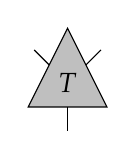
\begin{tikzpicture}
\begin{pgfonlayer}{foreground}
\draw[fill=lightgray] (0-0.5cm,0-0.3cm) -- (0,0+0.7cm) -- (0+0.5cm,0-0.3cm) -- cycle;
\node at (0,0) {$T$};
\end{pgfonlayer}
\begin{pgfonlayer}{background}
\draw[-] (0,0) -- (45:0.6cm);
\draw[-] (0,0) -- (135:0.6cm);
\draw[-] (0,0) -- (270:0.6cm);
\end{pgfonlayer}
\end{tikzpicture}
%
\end{minipage}
\end{center}

\end{changemargin}


%
\begin{changemargin}{20pt}{20pt}

\begin{center}
\begin{minipage}{.2\textwidth}
%
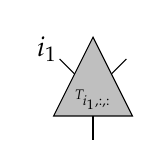
\begin{tikzpicture}
\begin{pgfonlayer}{foreground}
\draw[fill=lightgray] (0-0.5cm,0-0.3cm) -- (0,0+0.7cm) -- (0+0.5cm,0-0.3cm) -- cycle;
\node at (0,0-0.1) {\tiny$T_{i_{1},:,:}$};
\end{pgfonlayer}
\begin{pgfonlayer}{background}
\draw[-] (0,0) -- (45:0.6cm);
\draw[-] (0,0) -- (135:0.6cm);
\node at (137:0.8cm) {$i_{1}$};
\draw[-] (0,0) -- (270:0.6cm);
\end{pgfonlayer}
\end{tikzpicture}
%
\end{minipage}
%
\begin{minipage}{.2\textwidth}
%
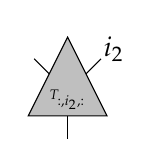
\begin{tikzpicture}
\begin{pgfonlayer}{foreground}
\draw[fill=lightgray] (0-0.5cm,0-0.3cm) -- (0,0+0.7cm) -- (0+0.5cm,0-0.3cm) -- cycle;
\node at (0,0-0.1) {\tiny$T_{:,i_{2},:}$};
\end{pgfonlayer}
\begin{pgfonlayer}{background}
\draw[-] (0,0) -- (45:0.6cm);
\node at (43:0.8cm) {$i_{2}$};
\draw[-] (0,0) -- (135:0.6cm);
\draw[-] (0,0) -- (270:0.6cm);
\end{pgfonlayer}
\end{tikzpicture}
%
\end{minipage}
%
\begin{minipage}{.2\textwidth}
%
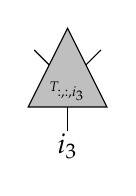
\begin{tikzpicture}
\begin{pgfonlayer}{foreground}
\draw[fill=lightgray] (0-0.5cm,0-0.3cm) -- (0,0+0.7cm) -- (0+0.5cm,0-0.3cm) -- cycle;
\node at (0,0-0.1) {\tiny$T_{:,:,i_{3}}$};
\end{pgfonlayer}
\begin{pgfonlayer}{background}
\draw[-] (0,0) -- (45:0.6cm);
\draw[-] (0,0) -- (135:0.6cm);
\draw[-] (0,0) -- (270:0.6cm);
\node at (270:0.8cm) {$i_{3}$};
\end{pgfonlayer}
\end{tikzpicture}
%
\end{minipage}
\end{center}

\end{changemargin}
%

\begin{changemargin}{20pt}{20pt}

\begin{center}
\begin{minipage}{.2\textwidth}
%
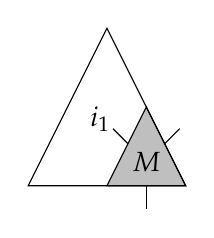
\begin{tikzpicture}
\begin{pgfonlayer}{foreground}
\draw[fill=lightgray] (0-0.5cm,0-0.3cm) -- (0,0+0.7cm) -- (0+0.5cm,0-0.3cm) -- cycle;
\node at (0,0) {$M$};
\draw (0-1.5cm,0-0.3cm) -- (0-0.5,0+1.7cm) -- (0+0.5cm,0-0.3cm) -- cycle;
\end{pgfonlayer}
\begin{pgfonlayer}{background}
\draw[-] (0,0) -- (45:0.6cm);
\draw[-] (0,0) -- (135:0.6cm);
\node at (137:0.8cm) {$i_{1}$};
\draw[-] (0,0) -- (270:0.6cm);
\end{pgfonlayer}
\end{tikzpicture}
%
\end{minipage}
%
\begin{minipage}{.2\textwidth}
%
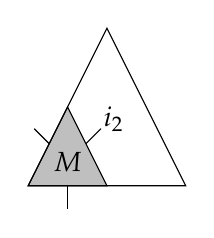
\begin{tikzpicture}
\begin{pgfonlayer}{foreground}
\draw[fill=lightgray] (0-0.5cm,0-0.3cm) -- (0,0+0.7cm) -- (0+0.5cm,0-0.3cm) -- cycle;
\node at (0,0) {$M$};
\draw (0-0.5cm,0-0.3cm) -- (0+1.5cm,0-0.3cm) -- (0+0.5cm,0+1.7cm) -- (0-0.5cm,0-0.3cm) -- cycle;
\end{pgfonlayer}
\begin{pgfonlayer}{background}
\draw[-] (0,0) -- (45:0.6cm);
\node at (43:0.8cm) {$i_{2}$};
\draw[-] (0,0) -- (135:0.6cm);
\draw[-] (0,0) -- (270:0.6cm);
\end{pgfonlayer}
\end{tikzpicture}
%
\end{minipage}
%
\begin{minipage}{.2\textwidth}
%
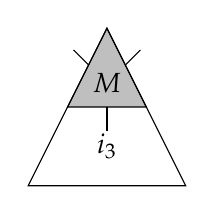
\begin{tikzpicture}
\begin{pgfonlayer}{foreground}
\draw[fill=lightgray] (0-0.5cm,0-0.3cm) -- (0,0+0.7cm) -- (0+0.5cm,0-0.3cm) -- cycle;
\node at (0,0) {$M$};
\draw (0,0+0.7cm) -- (0-1cm,0-1.3cm) -- (0+1cm,0-1.3cm) -- cycle;
\end{pgfonlayer}
\begin{pgfonlayer}{background}
\draw[-] (0,0) -- (45:0.6cm);
\draw[-] (0,0) -- (135:0.6cm);
\draw[-] (0,0) -- (270:0.6cm);
\node at (270:0.8cm) {$i_{3}$};
\end{pgfonlayer}
\end{tikzpicture}
%
\end{minipage}
\end{center}

\end{changemargin}

\newpage
\begin{changemargin}{0pt}{0pt}
Das bedeutet umgekehrt, man kann jeden d-Stufigen Tensor T auch auffassen als einen (d+k)-stufigen Tensor S,
bei dem k Moden mit festen Labeln $i_{j} \in I_{j}$ für $j = d+1,\dots,k$ versehen sind. 
Genauso wie man einen Vektor $v \in \mathbb{R}^{n}$ als Spalte $M_{\_,j}$ einer Matrix 
$M_{i,j} \in \mathbb{R}^{m\times n}$ auffassen kann.
\end{changemargin}

\begin{changemargin}{20pt}{20pt}
\begin{center}
%
\begin{minipage}{.2\textwidth}
% tensor T 5 modes
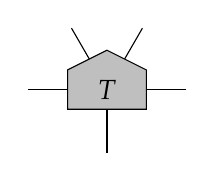
\begin{tikzpicture}
\begin{pgfonlayer}{foreground}
\draw[fill=lightgray] (0-0.5cm,0-0.25cm) -- (0+0.5cm,0-0.25cm) -- (0+0.5cm,0+0.25cm) -- (0,0+0.5cm) -- (0-0.5cm,0+0.25cm) -- cycle;
\node at (0,0) {$T$};
\end{pgfonlayer}
\begin{pgfonlayer}{background}
\draw[-] (0,0) -- (0:1cm);
\draw[-] (0,0) -- (1*60:0.9cm);
\draw[-] (0,0) -- (2*60:0.9cm);
\draw[-] (0,0) -- (180:1cm);
\draw[-] (0,0) -- (270:0.8cm);
\end{pgfonlayer}
\end{tikzpicture}
\end{minipage}
%
\begin{minipage}{.2\textwidth}
% tensor S inside of T
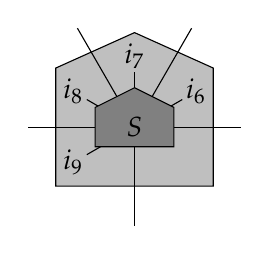
\begin{tikzpicture}
\begin{pgfonlayer}{foreground}
\draw[fill=gray] (0-0.5cm,0-0.25cm) -- (0+0.5cm,0-0.25cm) -- (0+0.5cm,0+0.25cm) -- (0,0+0.5cm) -- (0-0.5cm,0+0.25cm) -- cycle;
\node at (0,0) {$S$};
\end{pgfonlayer}
\draw[-] (0,0) -- (0:1.35cm);
\draw[-] (0,0) -- (1*60:1.45cm);
\draw[-] (0,0) -- (2*60:1.45cm);
\draw[-] (0,0) -- (180:1.35cm);
\draw[-] (0,0) -- (270:1.25cm);
\begin{pgfonlayer}{background}
\draw[fill=lightgray] (0-1cm,0-0.75cm) -- (0+1cm,0-0.75cm) -- (0+1cm,0+0.75cm) -- (0,0+1.2cm) -- (0-1cm,0+0.75cm) -- cycle;
\draw[-] (0,0) -- (1*30:0.7cm);
\node  at (1*30:0.9cm) {$i_{6}$};
\draw[-] (0,0) -- (3*30:0.7cm);
\node  at (3*30:0.9cm) {$i_{7}$};
\draw[-] (0,0) -- (5*30:0.7cm);
\node  at (5*30:0.9cm) {$i_{8}$};
\draw[-] (0,0) -- (7*30:0.7cm);
\node  at (7*30:0.9cm) {$i_{9}$};
\end{pgfonlayer}
\end{tikzpicture}
\end{minipage}
%
\end{center}
\end{changemargin}
$
T
\begin{pmatrix}[c]
i_{1}, i_{2}, i_{3}, i_{4}, i_{5}
\end{pmatrix}
=
S
\begin{pmatrix}[c]
i_{1}, i_{2}, i_{3}, i_{4}, i_{5}, \overline{i_{6}}, \overline{i_{7}}, \overline{i_{8}}, \overline{i_{9}}
\end{pmatrix}$ für feste $\overline{i_{j}} \in I_{j}, j\in\{6,\dots,9\}$.

\end{itemize}


% Formale Definition
\subsubsection{Formale Definition eines Tensors: Multi-Index, \textit{d}-stufiger Tensorraum}
\begin{changemargin}{0pt}{0pt}
\begin{definition}
Gegeben für $j \in \{1,\dots , d \}$ seien endliche Indexmengen
$I_{j} = \{1,\dots , n_{j} \}$.\\
Das kartesische Produkt dieser Mengen ergibt eine neue Indexmenge $\mathbf{I} := I_{1} \times \dots \times I_{d} \subset \mathbb{N}^{d}.$
Die Elemente $\mathbf{i}$ von $\mathbf{I}$ sind \underline{\textit{Multi-Indizes}} oder \underline{\textit{d-Tupel}}
$\mathbf{i} = (i_{1},\dots , i_{d})$ mit $i_{j} \in I_{j}$.

Auf dieser Indexmenge gibt es eine Halbordnung $\leq$, z.b. ist $(2,2,3,2,1) \leq (3,3,3,3,3)$.

Im Allgemeinen kann man zu jeder Indexmenge $J$ den Vektorraum $\mathbb{R}^{J}$ definieren als\\
$\mathbb{R}^{J} := \{ v = (v_{i})_{i \in J} : v_{i} \in \mathbb{R} \} := \{v : J \rightarrow \mathbb{R}; i \mapsto v_{i} \}$
(mit punktweiser Addition und skalarer Multiplikation). Dieser hat dann die Dimension
$\text{dim } \mathbb{R}^{J} = \#J$.\\
Für $J=\{1,\dots,n\}$ schreiben wir statt $\mathbb{R}^{\{1,\dots,n\}}$ kurz $\mathbb{R}^{n}$

Entsprechend für die Indexmenge $\mathbf{I}$ definieren wir den Vektorraum

\begin{equation} \label{eq:1.1}
\mathbb{R}^{\mathbf{I}} = \{\mathbf{v} = (\mathbf{v[i]})_{\mathbf{i} \in \mathbf{I}} : \mathbf{v}[i_{1},\dots,i_{d}] \in \mathbb{R} \}
\end{equation}

mit Dimension $\#\mathbf{I} = \prod_{j=1}^{d} \#I_{j} = \prod_{j=1}^{d} n_{j}$.

Diesen Raum nennen wir \underline{\textit{Tensorraum der Ordnung $d$}} und seine Elemente heißen\\
\underline{\textit{$d$-stufige Tensoren}}. Die einzelnen $j \in \{1,\dots,d\}$ nennen wir \underline{\textit{j-te Mode}}. \\
\end{definition}

\begin{rmk}
Im Fall von $n_{1} = n_{2} = \dots = n_{d} =: n$ (man spricht dann von einem \textit{kubischen} Tensor) ist
$\text{dim } \mathbb{R}^{\mathbf{I}} = n^{d}$, was für etwas größere $n$ und $d$ schon
eine sehr große Zahl wird. Da $\mathbb{R}^{\mathbf{I}}$ der Raum aller möglichen Tensoren mit Multi-Indizes in $\mathbf{I}$ ist, gibt es bei
größerer Dimension, z.B. $n = 1000, d = 20$ also $n^{d} = 1000^{20} = 10^{60}$, sehr viel leeren Raum, d.h. es ist schwierig, signifikante Daten zu
bekommen. Dieses Problem kennt man unter dem Namen \textit{Curse of Dimensionality}, also \textit{Fluch der Dimensionalität}.\\
Ein Thema dieses Vortrages ist, Teilräume von $\mathbb{R}^{\mathbf{I}}$ zu konstruieren mit beschränkter Dimension.
\end{rmk}
\end{changemargin}

\newpage
%1.1.3 Tensorprodukt
\subsubsection{Das Tensorprodukt $\otimes$ als Beziehung zwischen $\mathbb{R}^{\mathbf{I}}$ und den $\mathbb{R}^{I_{j}}$}
\begin{changemargin}{0pt}{0pt}

\begin{definition}
Für Vektoren $v^{(j)} \in \mathbb{R}^{I_{j}} \hspace{1mm}(1 \leq j \leq d)$ definieren wir das \textit{Tensorprodukt}

\[\mathbf{v} := v^{(1)} \otimes v^{(2)} \otimes \dots \otimes v^{(d)} = \bigotimes^{d}_{j=1} v^{(j)} \in \mathbb{R}^{\mathbf{I}}\]

durch ihre Einträge

\begin{equation} \label{eq:1.2}
\mathbf{v}_{\mathbf{i}} = \mathbf{v}[\mathbf{i}] = \mathbf{v}[i_{1},\dots,i_{d}] 
= v^{(1)}_{i_{1}} \cdot  v^{(2)}_{i_{2}} \cdot \hspace{0.5mm}_{\dots} \cdot  v^{(d)}_{i_{d}} \text{ für alle } \mathbf{i} \in \mathbf{I}.
\end{equation}

Solche Produkte $v^{(1)} \otimes v^{(2)} \otimes \dots \otimes v^{(d)}$ heißen \textit{elementare Tensoren}.
\end{definition}

Ein allgemeiner Tensor $\mathbf{v} \in \mathbb{R}^{\mathbf{I}}$ ist meist nicht durch ein einzelnes Tensorprodukt darstellbar,
sondern als Linearkombination von elementaren Tensoren.

\[ \mathbf{v} = \sum_{k=1}^{n} \bigotimes_{j=1}^{d} v^{(j)}_{k}\]

\[= v_{1}^{(1)} \otimes v_{1}^{(2)} \otimes \dots \otimes v_{1}^{(d)} + v_{2}^{(1)} \otimes v_{2}^{(2)} \otimes
\dots \otimes v_{2}^{(d)} +\dots
+v_{n}^{(1)} \otimes v_{n}^{(2)} \otimes \dots \otimes v_{n}^{(d)}  \]

\end{changemargin}

\begin{rmk}[Einschub: Tensorprodukt bei Octave / Matlab]
\begin{changemargin}{0pt}{0pt}
In Octave kann man mit der Funktion \texttt{kron} aus mehreren Vektoren das Kronecker-Produkt bilden, und die daraus
entstandene Matrix dann mit der Funktion \texttt{reshape} in ein mehrdimensionales Zahlenfeld umwandeln. Mehrere
Tensoren kann man dann addieren.
\end{changemargin}

\begin{changemargin}{15pt}{15pt}
\small\texttt{\noindent
u1 = [1,0,1,1,2]; v1 = [0,1,2,0,3]; w1 = [1,0,0,1,0];\\
u2 = [4,0,3]; v2 = [0,1,0]; w2 = [2,2,3];\\
u3 = [0,1,4,2]; v3 = [1,5,7,6]; w3 = [8,1,0,0];\\
u4 = [1,1]; v4 = [1,2]; w4 = [0,1];\\
U = reshape( kron(u1,u2,u3,u4), [length(u1) length(u2) length(u3) length(u4)] )\\
V = reshape( kron(v1,v2,v3,v4), [length(v1) length(v2) length(v3) length(v4)] )\\
W = reshape( kron(w1,w2,w3,w4), [length(w1) length(w2) length(w3) length(w4)] )\\
T = U+V+W}
\end{changemargin}

Bei der praktischen Verwendung hat sich aber gezeigt, dass die Funktion \texttt{kron} eine sehr
unintuitive Sortierung der Moden vornimmt, was vor allem die Multiplikation Matrix x Tensor schwierig
macht. Im proprietären Paket \texttt{tensortoolbox} \cite{tensortools} findet sich auch eine Funktion
ttm.m welche die Moden permutiert.
\end{rmk}

\begin{changemargin}{0pt}{0pt}
Das Tensorprodukt verwenden wir auf Vektorräume bezogen durch folgende Darstellung:

\begin{definition}
Das \underline{\textit{Tensorprodukt}} der Vektorräume $\mathbb{R}^{I_{j}}$ ist definiert als
\begin{equation}
\bigotimes^{d}_{j=1} \mathbb{R}^{I_{j}} := span \{ v^{(1)} \otimes v^{(2)} \otimes \dots \otimes v^{(d)} : v^{(j)} \in \mathbb{R}^{I_{j}},
1\leq j \leq d \},
\end{equation} also die Menge der endlichen Linearkombinationen von Elementar-Tensoren.
\end{definition}

\newpage
\begin{lemma}
Es gilt $\bigotimes^{d}_{j=1} \mathbb{R}^{I_{j}} = \mathbb{R}^{\mathbf{I}}$.
\end{lemma}

\begin{proof}[\underline{Beweis:}\nopunct]
Bezeichnet man die kanonischen Einheitsvektoren im $\mathbb{R}^{n_{j}}$ mit $\mathbf{e}_{j,k}, 1\leq k\leq n_{j}$, so ist
die $\prod^{d}_{j=1} n_{j}$-elementige Menge

\[ \{\mathbf{e}_{1,k_{1}}\otimes \dots \otimes \mathbf{e}_{d,k_{d}} : 1\leq k_{j} \leq n_{j}, 1\leq j\leq d\} \]

ein Erzeugendensystem von $\bigotimes^{d}_{j=1} \mathbb{R}^{n_{j}}$. Es ist sogar linear unabhängig, denn seien die\\
Koeffizienten
$\lambda_{k_{1},\dots,k_{d}} \in \mathbb{R}$ sodass

\[ \sum_{1\leq k_{1}\leq n_{1}} \dots \sum_{1\leq k_{d}\leq n_{d}} \lambda_{k_{1},\dots,k_{d}} \mathbf{e}_{1,k_{1}} \otimes \dots
\otimes \mathbf{e}_{d,k_{d}} = \mathbf{0} \in \mathbb{R}^{\mathbf{I}} \]

d.h. komponentenweise mit $(\mathbf{e}_{1,k_{1}} \otimes \dots \otimes \mathbf{e}_{d,k_{d}})(\mathbf{i}) = \prod^{d}_{j=1} (\mathbf{e}_{j,k_{j}})_{i_j}$

\[ \sum_{1\leq k_{1}\leq n_{1}} \dots \sum_{1\leq k_{d}\leq n_{d}} \lambda_{k_{1},\dots,k_{d}}  \prod^{d}_{j=1} (\mathbf{e}_{j,k_{j}})_{i_j} = 0 \]

Wegen $(\mathbf{e}_{j,k_{j}})_{i_j} = \delta_{k_{j},i_{j}}$ bleibt von der linken Summe für festes $\mathbf{i} \in \mathbf{I}$ nur das Gewicht
$\lambda_{i_{1},\dots,i_{d}}$ übrig, d.h. $\lambda_{i_{1},\dots,i_{d}} = 0$ für alle $\mathbf{i} \in \mathbf{I}$.

\end{proof}

\end{changemargin}

%universalitaet Tensorprodukt
\subsubsection{Tensoren als Multilineare Abbildungen: Universalität des Tensorprodukts}
\begin{changemargin}{0pt}{0pt}

Eine Abblidung $\varphi : V_{1} \times \dots \times V_{d} \rightarrow U$ heißt \textit{\underline{multilinear}}, wenn sie in jedem Argument linear ist.

Seien $V_{j} \hspace{0.5mm} (1\leq j \leq d)$ und $U$ Vektorräume über $\mathbb{K}$. Dann \textit{existiert} für jede multilineare Abbildung
$\varphi : V_{1} \times \dots \times V_{d} \rightarrow U$

eine \underline{eindeutige} lineare Abbildung $\Phi : \bigotimes^{d}_{j=1} V_{j} \rightarrow U$ sodass

\[ \varphi(v^{(1)}, v^{(2)},\dots,v^{(d)}) = \Phi(v^{(1)} \otimes v^{(2)} \otimes \dots \otimes v^{(d)})\]

Dieser Sachverhalt lässt sich auch in folgendem \textit{kommutativen Diagramm} darstellen:

\begin{center}
\begin{minipage}{.33\textwidth}
\end{minipage}
\begin{minipage}{.33\textwidth}
%kommutierendes Dreiecks-Diagramm
\begin{xy}
%vertices
(10,35)*+{V_{1}\times\dots\times V_{d}}="o1";(35,35)*+{U}="o2";
(18,25)*+{\circlearrowleft};
(10,10)*+{\bigotimes^{d}_{j=1} V_{j}}="u1";
%arrows
{\ar@{->}_{\Phi} "u1";"o2"};%
{\ar@{->}^{\hspace{5mm}\varphi} "o1";"o2"};%
{\ar@{->}_{\otimes} "o1";"u1"};%
\end{xy}
\end{minipage}
\begin{minipage}{.33\textwidth}
\end{minipage}
\end{center}
\end{changemargin}

\newpage
%Beispiel d=2
\subsubsection{Beispiel $d=2$: Matrizen als Tensoren}
\begin{changemargin}{0pt}{0pt}

\[ I_{1} := \{1,\dots,4\}, I_{2} := \{1,\dots,3\} \hspace{4mm} \mathbb{R}^{\mathbf{I}} = \mathbb{R}^{4\times 3}\]

$
(m_{i,j})_{1 \leq i \leq 4, 1 \leq j \leq 3} =
\begin{pmatrix}[ccc]
  1 & 0 & 2 \\
  0 & 1 & 4 \\
  3 & -2 & -2 \\
  5 & -1 & 6
\end{pmatrix} =
\begin{pmatrix}[c]
  m_{1,\_} \\
  m_{2,\_} \\
  3m_{1,\_} -2m_{2,\_} \\
  5m_{1,\_} -m_{2,\_}
\end{pmatrix} =
\begin{pmatrix}[cc]
  1m_{1,\_} \\
  0m_{1,\_} \\
  3m_{1,\_} \\
  5m_{1,\_}
\end{pmatrix} +
\begin{pmatrix}[c]
  0m_{2,\_} \\
  1m_{2,\_} \\
  -2m_{2,\_} \\
  -m_{2,\_}
\end{pmatrix} \\
=
\begin{pmatrix}[c]
  1 \\
  0 \\
  3 \\
  5
\end{pmatrix} \otimes m_{1,\_} +
\begin{pmatrix}[c]
  0 \\
  1 \\
  -2 \\
  -1
\end{pmatrix} \otimes m_{2,\_} =
\begin{pmatrix}[c]
  1 \\
  0 \\
  3 \\
  5
\end{pmatrix} \otimes
\begin{pmatrix}[ccc]
  1 & 0 & 2 \\
\end{pmatrix} +
\begin{pmatrix}[c]
  0 \\
  1 \\
  -2 \\
  -1
\end{pmatrix} \otimes
\begin{pmatrix}[ccc]
  0 & 1 & 4
\end{pmatrix}
$

Die Matrix $m$ lässt sich nicht als Elementartensor, also Tensorprodukt von zwei Vektoren darstellen, sondern als Linearkombination zweier solcher
Tensorprodukte. Man hätte auch eine größere Summe aus 12 Tensorprodukten $e_{i} \otimes e'_{k} (1\leq i \leq 4, 1\leq k \leq 3)$ mit
Koeffizienten $m_{i,j}$ schreiben können

$ m = \sum^{4}_{i=1} \sum^{3}_{k=3} m_{i,j} \hspace{1mm} e_{i} \otimes e'_{k} $, aber zwei Vektoren waren ausreichend.

Den \textit{Rang} $r$ einer Matrix $m \in \mathbb{R}^{I\times J}$ kann man auch charakterisieren als die minimale Anzahl Vektoren
$a_{i} \in \mathbb{R}^{I}, b_{i} \in \mathbb{R}^{J}$ sodass
\[ m = \sum^{r}_{i=1} a_{i}b_{i}^{\top} \]
Die Matrix $m$ hat also einen Rang von 2.
\end{changemargin}

%d=3 Graustufen-Video als Tensor
\subsubsection{Beispiel $d=3$ : Graustufen-Film: Höhe $\times$ Breite $\times$ Zeit }
\begin{changemargin}{0pt}{0pt}

https://drive.google.com/file/d/1usBNBSfnPuy1S2Oy8-QQPusrvBmVTohl/view \cite{tucker_tensorsketch}

(In dem Paper geht es um verschiedene Algorithmen zur Komprimierung von Tensoren, u.a. auch Tucker-Algorithmus.)

\end{changemargin}

\section{Tensordarstellung und Tensorzerlegung}

%1.2 Die Menge R_r
\subsection{Tensorrang und die Menge $\mathcal{R}_{r}$}
\begin{changemargin}{0pt}{0pt}

Seien $V_{j} \hspace{1mm} (1\leq j \leq d)$ Vektorräume, die den Tensorraum $\mathbf{V} := \bigotimes^{d}_{j=1} V_{j}$ erzeugen. Alle Linearkombinationen
von $r$ elementaren Tensoren sind enthalten in der Menge

\[\mathcal{R}_{\otimes,r} := \mathcal{R}_{r} := \mathcal{R}_{r}(\mathbf{V}) := \left\{ \sum^{r}_{\nu=1} v^{(1)}_{\nu} \otimes \dots \otimes v^{(d)}_{\nu} : v^{(j)}_{\nu} \in V_{j} \right\} \hspace{6mm} (r \in \mathbb{N}_{0}).\]

\subsubsection{Rang eines Tensors}

Gilt für einen Tensor $\mathbf{v}$ dass

$ \mathbf{v} \in \mathcal{R}_{r}$ und für alle $n<r \hspace{2mm} \mathbf{v} \notin \mathcal{R}_{n}$, dann definieren wir dies als den

\textit{\underline{Rang}} des Tensors, auch \textit{\underline{Produktrang}} genannt,
 $\text{rank} \hspace{1mm} \mathbf{v} := \min\{ r \in \mathbb{N} \hspace{0.5mm} | \hspace{0.5mm} \mathbf{v} \in \mathcal{R}_{r} \}$.

Um diesen Rang zu bestimmen, benötigt man aber bereits eine gegebene Zerlegung von $\mathbf{v}$ als Linearkombination von Elementartensoren.

Hastad \cite{hastad} hat gezeigt, dass die Bestimmung des Tensorrangs ein NP-schweres Problem ist.

\begin{rmk} (Abgeschlossenheit von $\mathcal{R}_{\mathbf{r}}$)
\\$\mathcal{R}_{\otimes,1}$ ist abgeschlossen.
\\$\mathcal{R}_{\mathbf{r}}$ ist nicht abgeschlossen für d $\geq 3$ und $r \geq 2$
\end{rmk}

\begin{thm} (De Silva / Lim 2008) \cite{de_silva_lim}
\\Seien $n_{1},n_{2},n_{3} \geq 2$. Die Folge $\{\mathbf{T}^{(n)}\}_{n \in \mathbb{N}} \subset \mathbb{R}^{n_{1}\times n_{2} \times n_{3}}$
sei konvergent mit $\text{rank}_{\otimes}(\mathbf{T}^{(n)}) \leq 2$ und Limes $\mathbf{T}$. Falls $\text{rank}_{\otimes}(\mathbf{T}) \geq 3$, so ist
$\text{rank}_{\otimes}(\mathbf{T}) = 3,$ und es existieren linear unabhängige Vektoren $\mathbf{x}_{j},\mathbf{y}_{j} \in \mathbb{R}^{n_{j}}, j \in
 \{1,2,3\}$, mit
\[\mathbf{T} = \mathbf{x}_{1} \otimes \mathbf{x}_{2} \otimes \mathbf{y}_{3} + \mathbf{x}_{1} \otimes \mathbf{y}_{2} \otimes \mathbf{x}_{3}
+ \mathbf{y}_{1} \otimes \mathbf{x}_{2} \otimes \mathbf{x}_{3}\]

Zu einem solchen $\mathbf{T} \in \mathbb{R}^{n_{1}\times n_{2}\times n_{3}}$ ist eine solche approximierende Folge gegeben durch

\[ \mathbf{T}^{(n)} := n(\mathbf{x}_{1} + \frac{1}{n} \mathbf{y}_{1}) \otimes (\mathbf{x}_{2} + \frac{1}{n}\mathbf{y}_{2}) \otimes
 (\mathbf{x}_{3} + \frac{1}{n}\mathbf{y}_{3}) -n\mathbf{x}_{1}\otimes \mathbf{x}_{2} \otimes \mathbf{x}_{3},\hspace{4mm} n \in \mathbb{N}.\]
\end{thm}

\begin{proof}[\underline{Beweis:}\nopunct]
Wir überlegen uns zuerst, dass die Tensoren $\mathbf{T}^{(n)}$ gegen $\mathbf{T}$ konvergieren:

\[ \mathbf{T}^{(n)} =  n(\mathbf{x}_{1} + \frac{1}{n} \mathbf{y}_{1}) \otimes (\mathbf{x}_{2} + \frac{1}{n}\mathbf{y}_{2}) \otimes
 (\mathbf{x}_{3} + \frac{1}{n}\mathbf{y}_{3}) -n\mathbf{x}_{1}\otimes \mathbf{x}_{2} \otimes \mathbf{x}_{3} \]

\[= \mathbf{T} + \frac{1}{n}(\mathbf{x}_{1} \otimes \mathbf{y}_{2} \otimes \mathbf{y}_{3} + \mathbf{y}_{1} \otimes \mathbf{x}_{2}
 \otimes \mathbf{y3} + \mathbf{y}_{1} \otimes \mathbf{y}_{2} \otimes \mathbf{x}_{3}) + \frac{1}{n^{2}}\mathbf{y}_{1}\otimes \mathbf{y}_{2} \otimes
\mathbf{y}_{3}, \]

also $\norm{\mathbf{T}^{(n)} - \mathbf{T}}^{2}_{F} \leq Cn^{-2} \rightarrow 0$ für $n \rightarrow \infty$.

Wir zeigen die restlichen Behauptungen für den Spezialfall $n_{1} = n_{2} = n_{3} = 2.$ Dass dies reicht wurde von De Silva und Lim gezeigt.
Sei $\mathbf{T} = \lim_{n\rightarrow\infty} \mathbf{T}^{(n)} \in \mathbb{R}^{2\times 2\times 2}$ mit $ \text{rank}_{\otimes}(\mathbf{T})\geq 3$ und
o.B.d.A. $\mathbf{T}(:,:,1)$ nichtsingulär für alle $n \in \mathbb{N}$, und die Eigenwerte von $\mathbf{T}^{(n)}(:,:,2)\mathbf{T}^{(n)}(:,:,1)^{-1}$ sind
reell. Wegen der Stetigkeit der Eigenwerte in Abhängigkeit der Matrixeinträge sind dann auch die Eigenwerte von 
$\mathbf{T}(:,:,2)\mathbf{T}(:,:,1)^{-1}$ reell. Da $\text{rank}_{\otimes}(T)\geq 3,$ sind die Eigenwerte nach Satz 3.2 gleich, und $\mathbf{T}(:,:,1)$ 
und $\mathbf{T}(:,:,2)$ sind nicht proportional. Also ist $\mathbf{T}(:,:,2)\mathbf{T}(:,:,1)^{-1}$ ähnlich zu einem Jordanblock 
$(^{\lambda \hspace{1mm} 1}_{0 \hspace{1mm} \lambda})$ mit $\lambda \in \mathbb{R}$, o.B.d.A. sogar

\[ \mathbf{T}(:,:,2) = \begin{pmatrix}[cc] \lambda & 1 \\ 0 & \lambda \end{pmatrix} \mathbf{T}(:,:,1).\]

Da $\mathbf{T}(:,:,1)$ invertierbar, existieren linear unabhängige $\mathbf{u}_{1},\mathbf{u}_{2} \in \mathbb{R}^{2}$ und $\mathbf{v}_{1},
\mathbf{v}_{2} \in \mathbb{R}^{2}$ mit
\[ \mathbf{T}(:,:,1) = \mathbf{u}_{1}\otimes\mathbf{v}_{1}+\mathbf{u}_{2}\otimes\mathbf{v}_{2},\]
also hat
\[ \mathbf{T}(:,:,2) - \lambda\mathbf{T}(:,:,1) = \mathbf{e}_{1}\mathbf{e}_{2}^{\top}(\mathbf{u}_{1}\mathbf{v}_{1}^{\top} 
+ \mathbf{u}_{2}\mathbf{v}_{2}^{\top}) = \mathbf{e}_{1}(\mathbf{e}_{2}^{\top}\mathbf{u}_{1}\mathbf{v}_{1}
+ \mathbf{e}_{2}^{\top}\mathbf{u}_{2}\mathbf{v}_{2})^{\top} \]
Rang 1 (denn $\mathbf{e}_{2}^{\top}\mathbf{u}_{1}$ und $\mathbf{e}_{2}^{\top}\mathbf{u}_{2}$ verschwinden nicht gleichzeitig) und
\begin{align*} \mathbf{T} &= \mathbf{T}(:,:,1)\otimes \mathbf{e}_{1} + \mathbf{T}(:,:,2)\otimes \mathbf{e}_{2}\\
&= \mathbf{T}(:,:,1)\otimes(\mathbf{e}_{1}+\lambda\mathbf{e}_2) + \mathbf{e}_1\otimes(\mathbf{e}_{2}^{\top}\mathbf{u}_{1}\mathbf{v}_{1}
+ \mathbf{e}_{2}^{\top}\mathbf{u}_{2}\mathbf{v}_{2})\otimes \mathbf{e}_{2}\\
&= (\mathbf{u}_{1}\otimes \mathbf{v}_{1} + \mathbf{u}_{2}\otimes\mathbf{v}_{2})\otimes(\mathbf{e}_{1}+\lambda\mathbf{e}_{2})
+ \mathbf{e}_{1}\otimes(\mathbf{e}_{2}^{\top}\mathbf{u}_{1}\mathbf{v}_{1} + \mathbf{e}_{2}^{\top}\mathbf{u}_{2}\mathbf{v}_{2})\otimes
\mathbf{e}_{2}
\end{align*}

liefert eine Zerlegung aus drei Elementartensoren, d.h. $\text{rank}_{\otimes}(\mathbf{T}) = 3.$
\end{proof}

\end{changemargin}

% Tucker-Rang
\subsection{Tucker-Rang und Tucker-Zerlegung: Die Menge $\mathcal{T}_{\mathbf{r}}$}

\subsubsection{Unterräume $U_{j}$ und minimale Unterräume $U_{j}^{\min}$}
\begin{changemargin}{0pt}{0pt}

Für einen Tensorraum $\mathbf{V} = \bigotimes^{d}_{j=1} V_{j}$ und einen fixen Tensor $\mathbf{v} \in \mathbf{V}$ gibt es
Untervektorräume $U_{j} \subset V_{j}$ mit

\begin{equation}
\mathbf{v} \in \mathbf{U} := \bigotimes^{d}_{j=1} U_{j}.
\end{equation}

Davon den kleinsten Unterraum in der Mode $j$ nennen wir dann $U^{\min}_{j}(\mathbf{v})$ für $1\leq j\leq d$, und seine Dimension
$r_{j} := \dim(U_{j}^{\min}(\mathbf{v})).$

\begin{definition}($\mathcal{T}_{\mathbf{r}}$)
Sei $\mathbf{V} := \bigotimes^{d}_{j=1} V_{j}$ und ein fixes $\mathbf{r} := (r_{1},\dots,r_{d})\in \mathbb{N}^{d}_{0}$, dann setze

\begin{equation}
\mathcal{T}_{\mathbf{r}} := \mathcal{T}_{\mathbf{r}}(\mathbf{V}) := 
\left\{ \mathbf{v}\in \mathbf{V} : 
\begin{aligned}
\text{Es gibt Unterräume } U_{j} \subset V_{j} \text{ sodass }\\
\dim(U_{j}) = r_{j} \text{ und } \mathbf{v} \in \mathbf{U} := \bigotimes^{d}_{j=1} U_{j}
\end{aligned} 
\right\}
\end{equation}
\end{definition}

Wir sagen, ein Tensor $\mathbf{v} \in \mathcal{T}_{\mathbf{r}}$ habe eine $(r_{1},\dots,r_{d})$-\textit{\underline{Tensor-Unterraum-Darstellung}}
(engl. \textit{tensor subspace representation}).

\begin{definition} (\textbf{Tucker-Rang})
Das minimale $d$-Tupel $\mathbf{r} = (r_{1},\dots,r_{d})$ natürlicher Zahlen, für das $\mathbf{v} \in \mathcal{T}_{\mathbf{r}}$ gilt, nennen wir
\textit{\underline{Tucker-Rang}} von $\mathbf{v}$.
\end{definition}

\end{changemargin}

\subsection{Approximierung}
\begin{changemargin}{0pt}{0pt}

\begin{lemma} (schwach abgeschlossen)
Sei $\mathbf{V} = \hspace{2mm}_{\norm{\cdot}}\bigotimes^{d}_{j=1} V_{j}$ ein Banach-Tensorraum mit Norm nicht schwächer als $\norm{\cdot}_{\vee}$. Dann ist die Teilmenge $\mathcal{T}_{\mathbf{r}} \subset \mathbf{V}$ schwach abgeschlossen.
\end{lemma}
\begin{proof}[\underline{Beweis:}\nopunct]
Sei $\mathbf{v}_{n} \in \mathcal{T}_\mathbf{r}$ eine schwach konvergente Folge mit $\mathbf{v}_{n} \rightharpoonup \mathbf{v} \in \mathbf{V}$.
Aus $\mathbf{v}_{n} \in \mathcal{T}_\mathbf{r}$ folgt, dass $U^{\min}_{j}(\mathbf{v}_{n})$ eine Dimension kleiner oder gleich $r_{j}$ hat.
Es gilt $\dim(U^{min}_{j}(\mathbf{v}))\leq r_{j}$, und damit $\mathbf{v} \in \mathcal{T}_{\mathbf{r}}$.
\end{proof}

\begin{alg}
Alternating least squares ($\mathbf{ALS}$) für $r = 1$. \cite{tucker_tensorsketch}
\begin{tabbing}
\hspace*{5mm}\=\hspace*{5mm}\=\hspace*{5mm}\=\hspace{5mm}\=\hspace{1cm}\= \kill
$\mathbf{function }$ ALS \hspace{1mm} $(\mathbf{T} \in \mathbb{R}^{\mathbf{I}})$\\
\> choose nonzero starting values $x_{j} \in \mathbb{R}^{n_{j}}, j= 1,\dots,d$\\
\> $\mathbf{while}$ not converged $\mathbf{do}$\\
\> \> $\mathbf{for}$ \hspace{2mm} $k = 1,\dots,d$ \hspace{2mm} $\mathbf{do}$\\
\> \> \>solve the linear least squares problem\\
\> \> \> \> $x_{k} \leftarrow$ \> $\arg \min \norm{\mathbf{T} - x_{1}\otimes\dots x_{k-1}\otimes y \otimes x_{x+1} \dots
\otimes x_{d}}^{2}_{F}$\\
\> \> \> \> \> $y \in \mathbb{R}^{n_{k}}$\\
\> \> $\mathbf{end for}$\\
\> $\mathbf{end while}$\\
\> $\mathbf{return } (x_{1},\dots,x_{d})$\\
$\mathbf{end function}$
\end{tabbing}
\end{alg}

\end{changemargin}

\subsubsection{Beispiel: Tucker-Zerlegung eines 5-stufigen Tensors}
\begin{changemargin}{0pt}{0pt}
\begin{center}
%
% tensor T
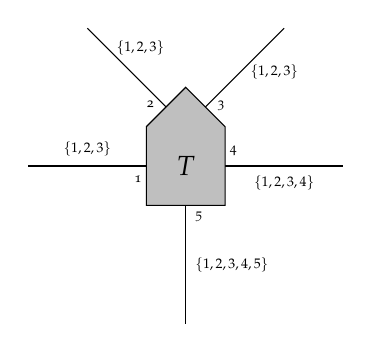
\begin{tikzpicture}
\begin{pgfonlayer}{foreground}
\draw[fill=lightgray] (0-0.5cm,0-0.5cm) -- (0+0.5cm,0-0.5cm) -- (0+0.5cm,0+0.5cm) -- (0,0+1cm) -- (0-0.5cm,0+0.5cm) -- cycle;
\node at (0,0) {$T$};
\end{pgfonlayer}
\begin{pgfonlayer}{background}
\draw[-] (0-0.5cm,0) -- node [below,pos=0.07] {\tiny1} node [above,midway] {\tiny$\{1,2,3\}$} (0-2cm,0); %j=1
\draw[-] (0-0.25cm,0+0.75cm) -- node [below,pos=0.2] {\tiny2} node [right,near end] {\tiny$\{1,2,3\}$} (0-1.25cm,0.5cm+1.25cm); %j=2
\draw[-] (0+0.25cm,0+0.75cm) -- node [below,pos=0.2] {\tiny3} node [right,pos=0.45] {\tiny$\{1,2,3\}$} (0+1.25cm,0.5cm+1.25cm); %j=3
\draw[-] (0+0.5cm,0) -- node [above,pos=0.07] {\tiny4} node [below,midway] {\tiny$\{1,2,3,4\}$} (0+2cm,0); %j=4
\draw[-] (0,0-0.5cm) -- node [right,pos=0.1] {\tiny5} node [right,midway] {\tiny$\{1,2,3,4,5\}$} (0,-0.5cm-1.5cm); %j=5
\end{pgfonlayer}
\end{tikzpicture}
\end{center}
$\mathbf{T} \in \mathbb{R}^{3\times3\times3\times4\times5}$ hat also $3\cdot3\cdot3\cdot4\cdot5 = 540$ Einträge.\\


\begin{center}
%
% core tensor X
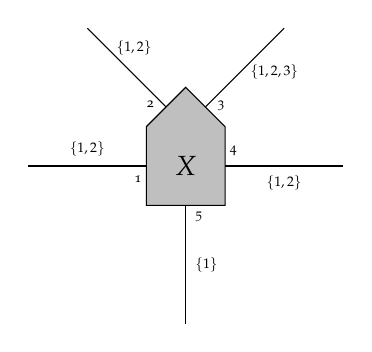
\begin{tikzpicture}
\begin{pgfonlayer}{foreground}
\draw[fill=lightgray] (0-0.5cm,0-0.5cm) -- (0+0.5cm,0-0.5cm) -- (0+0.5cm,0+0.5cm) -- (0,0+1cm) -- (0-0.5cm,0+0.5cm) -- cycle;
\node at (0,0) {$X$};
\end{pgfonlayer}
\begin{pgfonlayer}{background}
\draw[-] (0-0.5cm,0) -- node [below,pos=0.07] {\tiny1} node [above,midway] {\tiny$\{1,2\}$} (0-2cm,0); %j=1
\draw[-] (0-0.25cm,0+0.75cm) -- node [below,pos=0.2] {\tiny2} node [right,near end] {\tiny$\{1,2\}$} (0-1.25cm,0.5cm+1.25cm); %j=2
\draw[-] (0+0.25cm,0+0.75cm) -- node [below,pos=0.2] {\tiny3} node [right,pos=0.45] {\tiny$\{1,2,3\}$} (0+1.25cm,0.5cm+1.25cm); %j=3
\draw[-] (0+0.5cm,0) -- node [above,pos=0.07] {\tiny4} node [below,midway] {\tiny$\{1,2\}$} (0+2cm,0); %j=4
\draw[-] (0,0-0.5cm) -- node [right,pos=0.1] {\tiny5} node [right,midway] {\tiny$\{1\}$} (0,-0.5cm-1.5cm); %j=5
\end{pgfonlayer}
\end{tikzpicture}
\end{center}
Angenommen $\mathbf{T}$ hat eine Tucker-Zerlegung in einen Kern-Tensor $\mathbf{X} \in \mathbb{R}^{2\times2\times3\times2\times1}$ und die fünf
Matrizen $U_{1},\dots,U_{5}$.


\begin{center}
% 
% core tensor X with matrices U1,...,U5
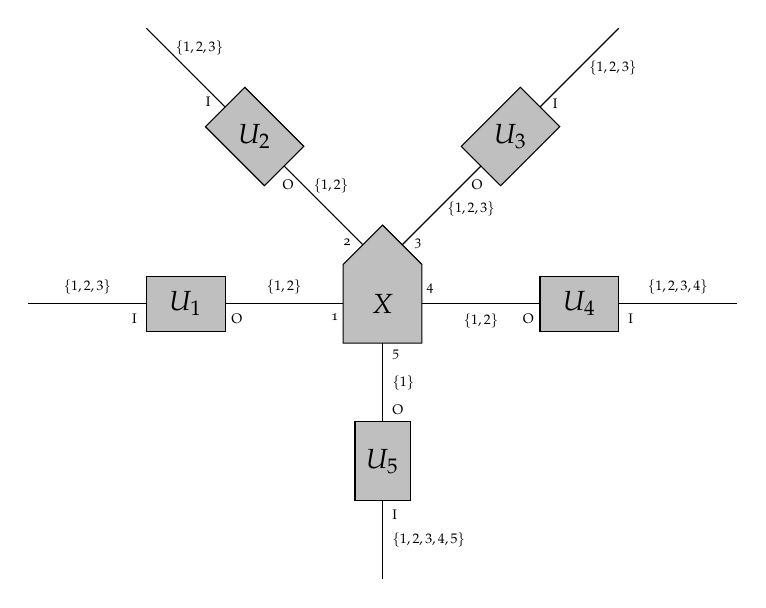
\begin{tikzpicture}
\begin{pgfonlayer}{foreground}
\draw[fill=lightgray] (0-0.5cm,0-0.5cm) -- (0+0.5cm,0-0.5cm) -- (0+0.5cm,0+0.5cm) -- (0,0+1cm) -- (0-0.5cm,0+0.5cm) -- cycle;
\node at (0,0) {$X$};
\end{pgfonlayer}
\begin{pgfonlayer}{background}
\draw[-] (0-0.5cm,0) -- node [below,pos=0.9] {\tiny O} node [below,pos=0.07] {\tiny1} node [above,midway] {\tiny$\{1,2\}$} (0-2cm,0); %j=1
\draw[-] (0-0.25cm,0+0.75cm) -- node [below,pos=0.95] {\tiny O} node [below,pos=0.2] {\tiny2} node [right,near end] {\tiny$\{1,2\}$}
 (0-1.25cm,0.5cm+1.25cm); %j=2
\draw[-] (0+0.25cm,0+0.75cm) -- node [below,pos=0.95] {\tiny O} node [below,pos=0.2] {\tiny3} node [right,pos=0.45] {\tiny$\{1,2,3\}$} 
(0+1.25cm,0.5cm+1.25cm); %j=3
\draw[-] (0+0.5cm,0) -- node [below,pos=0.9] {\tiny O} node [above,pos=0.07] {\tiny4} node [below,midway] {\tiny$\{1,2\}$} 
(0+2cm,0); %j=4
\draw[-] (0,0-0.5cm) -- node [right,pos=0.85] {\tiny O} node [right,pos=0.15] {\tiny5} node [right,midway] {\tiny$\{1\}$} 
(0,-0.5cm-1cm); %j=5
\end{pgfonlayer}
%U1 p=(-2.5cm,0)
\draw[fill=lightgray] (-2.5cm-0.5cm,0-0.35cm) -- (-2.5cm+0.5cm,0-0.35cm) -- (-2.5cm+0.5cm,0+0.35cm) -- (-2.5cm-0.5cm,0+0.35cm) -- cycle;
\node at (-2.5cm,0) {$U_{1}$};
\draw[-] (-2.5cm-0.5cm,0) -- node [below,pos=0.1] {\tiny I} node [above,midway] {\tiny$\{1,2,3\}$} (-2.5cm-2cm,0);
%U2 p=(-1.5cm,2cm)
\draw[fill=lightgray] (-1.5cm,2cm-0.5cm) -- (-1.5cm-0.75cm,2cm-0.5cm+0.75cm) -- (-1.5cm-0.25cm,2cm+0.75cm) -- (-1.5cm+0.5cm,2cm) -- cycle;
\node at (-1.5cm-0.125cm,2cm+0.125cm) {$U_{2}$};
\draw[-] (-2cm,2.5cm) -- node [left,pos=0.06] {\tiny I} node [right,near end] {\tiny$\{1,2,3\}$} (-3cm,3.5cm);
%U3 p=(1.5cm,2cm)
\draw[fill=lightgray] (1.5cm-0.5cm,2cm) -- (1.5cm+0.25cm,2cm+0.75cm) -- (1.5cm+0.75cm,2cm+0.25cm) -- (1.5cm,2cm-0.5cm) -- cycle;
\node at (1.5cm+0.125cm,2cm+0.125cm) {$U_{3}$};
\draw[-] (1.5cm+0.5cm,2cm+0.5cm) -- node [right,pos=0.04] {\tiny I} node [right,midway] {\tiny$\{1,2,3\}$} (3cm,3.5cm);
%U4 p=(2.5cm,0)
\draw[fill=lightgray] (2.5cm-0.5cm,0-0.35cm) -- (2.5cm+0.5cm,0-0.35cm) -- (2.5cm+0.5cm,0+0.35cm) -- (2.5cm-0.5cm,0+0.35cm) -- cycle;
\node at (2.5cm,0) {$U_{4}$};
\draw[-] (2.5cm+0.5cm,0) -- node [below,pos=0.1] {\tiny I} node [above,pos=0.5] {\tiny$\{1,2,3,4\}$} (2.5cm+2cm,0);
%U5 p=(0,-2cm)
\draw[fill=lightgray] (0-0.35cm,-2cm+0.5cm) -- (0-0.35cm,-2cm-0.5cm) -- (0+0.35cm,-2cm-0.5cm) -- (0+0.35cm,-2cm+0.5cm) -- cycle;
\node at (0,-2cm) {$U_{5}$};
\draw[-] (0,-2.5cm) -- node [right,pos=0.18] {\tiny I}  node [right,midway] {\tiny$\{1,2,3,4,5\}$} (0,-3.5cm);
\end{tikzpicture}
\end{center}

wobei $X \in \mathbb{R}^{2\times 2\times 3\times 2\times 1}$ d.h. es gibt $2\cdot 2\cdot 3\cdot 2\cdot 1 = 24$ Einträge zu speichern,
dazu noch die Einträge in den Matrizen $3\cdot2 + 3\cdot2 + 3\cdot3 + 2\cdot4 +1\cdot5 = 34$ macht insgesamt $24+34=58$ Einträge
statt $540$. Dass man denselben Datengehalt in so viel weniger Platz darstellen kann, macht deutlich, dass unter den 
540 möglichen Einträgen viel leerer Raum war. Zum Beispiel konnte bei der fünften Mode die $5 \times 1$-Matrix 
$\mathcal{U}_{5}$ vom Rang 1 faktorisiert werden, was die Dimension schon durch 5 teilt.


\end{changemargin}

\newpage

\begin{thebibliography}{9}
\bibitem{tensor_skript_raasch}
Tensor\_Skript\_Numerische multilineare Algebra- Thorsten Raasch

\bibitem{hackbusch}
(Springer Series in Computational Mathematics 42) Wolfgang Hackbusch (auth.):
Tensor Spaces and Numerical Tensor Calculus. 42-Springer-Verlag Berlin Heidelberg (2012)

\bibitem{hastad}
Hastad, J.: Tensor rank is NP-complete. J. Algorithms 11, 644–654 (1990)

\bibitem{de_silva_lim}
Vin de Silva and Lek-Heng Lim:
Tensor Rank and the Ill-Posedness of the Best Low-Rank Approximation Problem

Read More: \texttt{https://epubs.siam.org/doi/10.1137/06066518X}

\bibitem{tucker_tensorsketch}
Stephen Becker and  Osman Asif Malik: Low-rank Tucker decomposition of large tensors using
TensorSketch,
\\\texttt{http://amath.colorado.edu/faculty/becker/TensorSketch.pdf}
\\\texttt{https://drive.google.com/file/d/1usBNBSfnPuy1S2Oy8-QQPusrvBmVTohl/view}

\bibitem{tensor_networs_simons}
Simons Institute: Mini Crash Course: Tensor Networks,
\\\texttt{https://www.youtube.com/watch?v=YN2YBB0viKo}

\bibitem{tensortools}
\texttt{https://www.tensortoolbox.org/}

\end{thebibliography}

\end{document}